
\documentclass[12pt,epsfig,color,russian]{article}
\usepackage[russian]{babel}
\usepackage{epsfig}
\usepackage{color}

\topmargin=0cm
\hoffset -30mm
\voffset -12mm
\setlength{\unitlength}{1mm}
\parindent=10mm
\textheight=250mm
\textwidth=185mm
\pagestyle{empty}

\begin{document}
\sf\Large
\centerline{\LARGE\bf Основы ТЕРМОДИНАМИКИ}
\underline{Молекулярно-кинетическое} описание вещества (уже изучили).\\
\underline{Макроскопические} физические величины (давление, температура, etc.) -- это средние характеристики по большому числу атомов или молекул (давление = передача импульса при ударах молекул о стенки;\\
 температура = кинетическая энергия на степень свободы).

СЛУЧАЙНЫЙ характер (беспорядочность) движения молекул $\Rightarrow$ ста\-ти\-с\-ти\-че\-с\-кие закономерности. Распределение Максвелла; распределение Больцмана. На микро-уровне бывают флуктуации (броуновское движение), но в целом статистика работает верно $\Rightarrow$ раздел теоретической физики \underline{СТАТИСТИЧЕСКАЯ ФИЗИКА.}

Другой подход: не вникая в суть микро-процессов, описывать МАКРО-характеристики явлений, а именно --- превращение ЭНЕРГИИ из одного вида в другой: \underline{ТЕРМОДИНАМИКА.}\\

\underline{\bf Начала термодинамики}: совокупность постулатов (они являются именно \underline{постулатами}, хотя и подтверждены экспериментально)
\begin{enumerate}
\setcounter{enumi}{-1}
\item (Общее) Замкнутая система независимо от начального состояния в конце концов приходит к состоянию термодинамического равновесия и самостоятельно выйти из него не может; все части системы при этом будут иметь одинаковую температуру.
\item Закон сохранения энергии в применении к термодинамическим системам (запрет вечного двигателя 1 рода).
\item Ограничения на направление термодинамических процессов (запрет на самопроизвольную передачу тепла от холодных тел к горячим) = (запрет вечного двигателя 2 рода) -- закон возрастания энтропии.
\item Регулирует поведение энтропии вблизи абсолютного нуля температуры ($\lim\limits_{T\rightarrow0}S=0$) --- теорема Нернста.
\end{enumerate}
\newpage
Ощущения тепла или холода -- субъективны, зависят не только от температуры, но и от теплопроводности, и от теплоемкости. Для измерения $T$ нужен контакт термометра с измеряемым телом. Тепло ``перетекает'' от горячего к холодному, как жидкость {\bf теплород} (идея XVIII века). Идея была неверная, но привела к развитию калори\-мет\-ри\-чес\-ких измерений (Георг Вильгельм Рихман, 1750, СПб, погиб в 1753 г. при экспериментах с атмосферным электричеством). Понятие о {\bf количестве тепла $\bf Q$}.\\
 \begin{picture}(185,75)(0,0)
 %\put(0,0){\framebox(185,70)[b]{}}
 \put(90,0){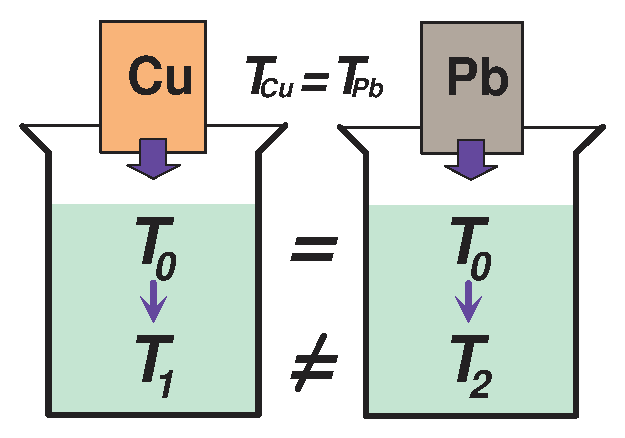
\includegraphics{GP012F01.eps}}
 \put(0,68){\makebox(0,0)[tl]{\parbox{85mm}{
 Если медный и свинцовый бру\-с\-ки одинаковой массы нагреть до одинаковой $T_{\rm Cu}$=$
 T_{\rm Pb}$=$T_i$ и опу\-с\-тить их в одинаковые сосуды с водой равной температуры $T_0$, то вода в них нагреется до \underline{\bf разной} $T_1\neq T_2$. Вывод: медь и свинец вмещают разное ко\-ли\-че\-с\-тво теплорода!!! (кол-во тепла $Q$)
 }}}
 \end{picture}\\
Так же выяснилось, что передаваемое при теплообмене количество тепла $\Delta Q \propto$ массе бруска $m$ и изменению температуры $\Delta T$:
\begin{displaymath}
\Delta Q = c\cdot m\cdot \Delta T\hspace{10mm}(c\texttt{ -- теплоемкость})
\end{displaymath}
Идея теплорода была очень удобна при вычислениях теплообмена, но не объясняла нагрева при трении (М.В.Ломоносов, 1744, СПб, на это указывал).

В начале XIX в. Румфорд (Benjamin Thompson, Count Rumford, London) и Дэви (Humphry Davy, London) показали, что нагрев при трении -- это факт. Джоуль (James Joule, 1843, Manchester) измерил количественно эту связь: 1 калория эквивалентна 4.18 Дж.

Принято говорить о механическом эквиваленте тепла, поскольку и тепло $Q$, и работа $A$ меняют внутреннюю энергию системы при ее переходе из одного состояния в другое. Поэтому в дальнейшем единицы измерения для $Q$ и $A$ будем использовать одни и те же.
\newpage
\noindent
Рассмотрим некую термодинамическую систему (газ в цилиндре с порш\-нем) в состоянии 1. Обозначим за $U_1$ ее внетреннюю энергию. Пусть над ней совершается какая-то работа $dA_1$ (мы сдавливаем поршень), и пусть ей путем прямого нагрева передается некое количество тепла $dQ_1$ (мы цилиндр еще и подогреваем). \\
 \begin{picture}(185,90)(0,0)
 %\put(0,0){\framebox(185,90)[b]{}}
 \put(15,0){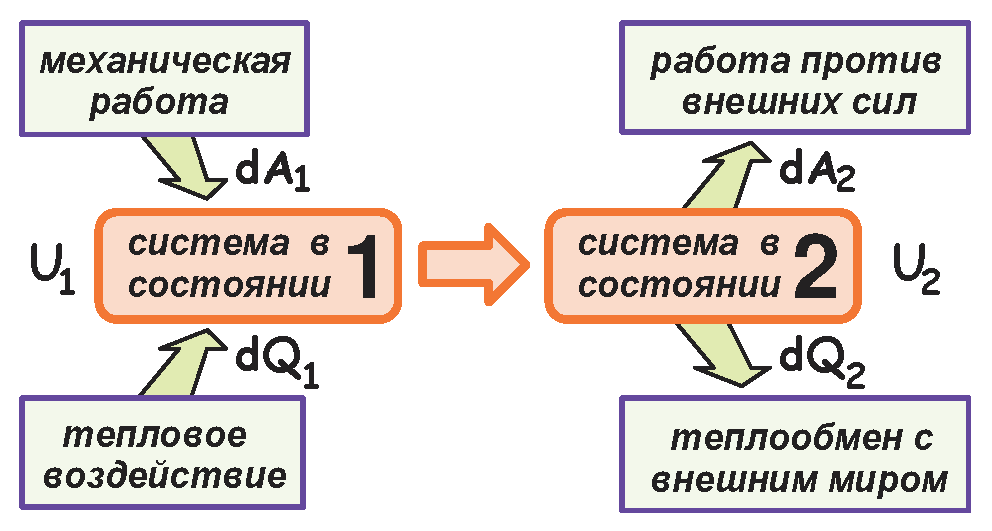
\includegraphics{GP012F02.eps}}
 \put(0,68){\makebox(0,0)[tl]{\parbox{85mm}{
 }}}
 \end{picture}\\
Внутренняя энергия системы при этом изменится на величину $dU=dA_1+dQ_1$. Поскольку не система совершила работу, а внешние силы, то $dA_1$>0. Внешний нагрев также означает $dQ_1$>0. Таким образом, оба эти воздействия УВЕЛИЧИЛИ энергию системы.

 Если затем система перейдет в состояние 2, отдав количество тепла $dQ_2$ в окружающее пространство (окружающий воздух нагрелся от контакта с цилиндром) и совершив работу $dA_2$ против внешних сил (поршень вер\-нул\-ся на прежнее место, преодолев наше сопротивление), то в итоге ее внутренняя энергия станет равной
\begin{displaymath}
U_2=U_1+dA_1+dQ_1-dA_2-dQ_2
\end{displaymath}
Здесь знаки ``--'' перед $dA_2$ и $dQ_2$ символизируют направление ПРОЧЬ ОТ СИСТЕМЫ, уменьшающее ее внутреннюю энергию.

Итак, {\bf изменение энергии системы при ее переходе из одного состояния в другое равно сумме механических экви\-ва\-лен\-тов всех внешних воздействий, ведущих к этому переходу}.

В изолированной системе внешних воздействий нет. При взаимо\-дей\-с\-т\-вии частей системы друг с другом $U$ системы сохраняется, хотя между частями энергия передается и переходит из одного вида в другой.\\
 \begin{picture}(185,60)(0,0)
 %\put(0,0){\framebox(185,60)[b]{}}
 \put(55,0){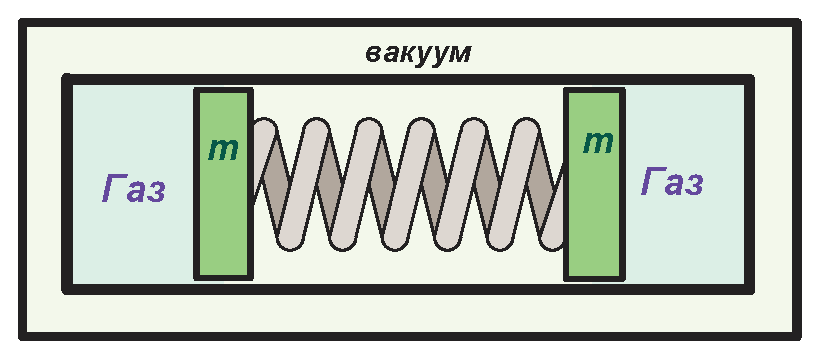
\includegraphics{GP012F03.eps}}
 \put(0,56){\makebox(0,0)[tl]{\parbox{50mm}{
\underline{Пример:}  в термосе на\-хо\-дит\-ся ци\-линдр с дву\-мя порш\-ня\-ми и пру\-жи\-ной. Пру\-жи\-на бы\-ла сжа\-та и сдер\-жи\-ва\-лась нит\-кой. Нитка лопнула!
 }}}
 \end{picture}\\
$E_p$ сжатой пружины передастся поршням и превратится в их $E_k$. Они сожмут газ, его давление возрастет и остановит поршни. При этом, вся $E_k$ поршней перейдет в $E_p$ сжатого газа. Газ толкнет остановившиеся поршни назад, и они сожмут пружину. И так далее. До бесконечности это длиться не будет: ведь даже если нет трения между поршнем и цилиндром, то есть внутреннее трение в газе! Из-за этого трения газ будет каждый раз немного нагреваться, пока вся первоначальная энергия пружины не пре\-вра\-тит\-ся в тепло. Ну, не вся, а почти вся. Ведь у {\bf нагретого} газа давление выше, и $\Rightarrow$ потенциальная энергия больше.\\

Равновесные и неравновесные системы.\\
 \begin{picture}(185,40)(0,0)
 %\put(0,0){\framebox(185,40)[b]{}}
 \put(170,0){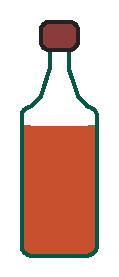
\includegraphics{GP012F04.eps}}
 \put(0,36){\makebox(0,0)[tl]{\parbox{165mm}{
 Равновесное состояние: параметры = const без постороннего влияния.
\underline{Пример:} закрытая бутылка с вином -- это 2-фазная равновесная система жидкости и насыщенных паров. Давление и температура в разных частях бутылки -- одинаковы и не меняются со временем. соотношение $m_L/m_G$ тоже постоянно.
 }}}
 \end{picture}

Откупоренная бутылка -- неравновесна. Жидкость все время испаряется.

\underline{Другой пример:} включенный паяльник -- неравновесная система. Его жало все время подогревается спиралью, а рукоятка охлаждается воздухом.

У выключенного паяльника жало остынет, температура везде сравняется, и система станет равновесной.

Любой процесс является изменением параметров и представляет собой ряд неравновесных состояний.
Равновесный процесс состоял бы из равно\-весных состояний и должен быть бесконечно медленным. Реально такого не бывает. Но если реальный (неравновесный) процесс разложить на очень малые кусочки, то в пределах одного кусочка можно считать систему равновесной. Тогда в каждый момент можно считать, что у системы есть определенные параметры ($p, V, T$), которые меняются плавно и непрерывно,\\
 \begin{picture}(185,60)(0,0)
 %\put(0,0){\framebox(185,60)[b]{}}
 \put(0,0){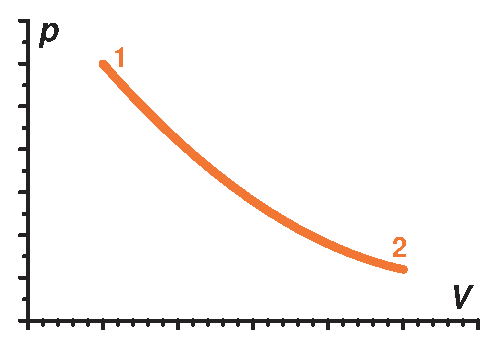
\includegraphics{GP012F05.eps}}
 \put(105,0){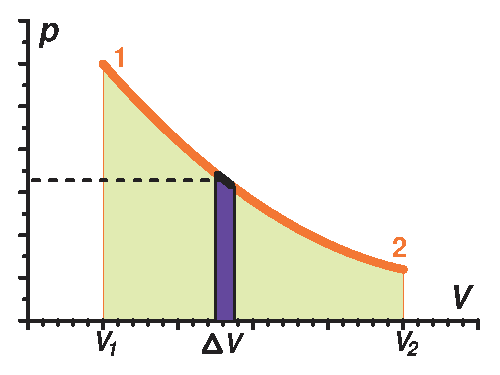
\includegraphics{GP012F06.eps}}
 \put(40,56){\makebox(0,0)[tl]{\parbox{45mm}{
и процесс можно изобразить линией
 }}}
 \put(39,39){\vector(-1,-1){8}}
 \end{picture}\\
 Если система переходит из состояния 1 в 2, то КАКАЯ совершится РАБОТА? При малом изменении $\Delta V$ работа будет $\Delta A=p\;\Delta V$, а на всем участке --
 \begin{displaymath}
 A_{1\rightarrow2}=\int\limits_{V_1}^{V_2}p(V)\;dV
 \end{displaymath}
 При этом, конечно, должен соблюдаться ЗСЭ, поэтому изменение полной энергии системы
 \begin{displaymath}
 \Delta U_{1\rightarrow2} = U_2-U_1=Q_{1\rightarrow2}-A_{1\rightarrow2}
 \end{displaymath}
 где $Q_{1\rightarrow2}$ -- это приток тепла в систему извне.

 Если мы хотим, чтобы энергия системы не изменилась, мы должны скомпенсировать совершенную ею работу соответствующим притоком тепла.\\

 Чтобы сделать не одноразовый фокус с расширением газа, а регулярно работающую {\bf тепловую машину}, нужен {\bf циклический процесс}. Цикл (круг) -- это такой процесс, после которого система возвращается в исходное состояние (все параметры принимают первоначальные значения).\\
\noindent
  \begin{picture}(185,200)(0,0)
 %\put(0,0){\framebox(185,200)[b]{}}
 \put(0,140){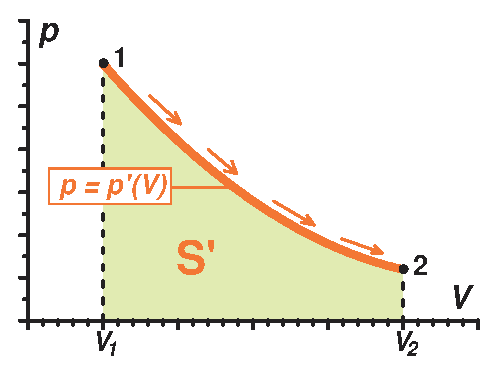
\includegraphics{GP012F07.eps}}
 \put(0,70){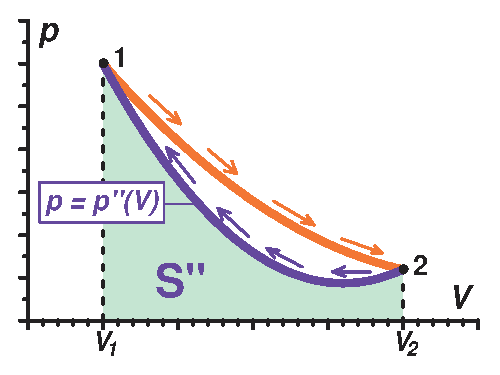
\includegraphics{GP012F08.eps}}
 \put(0,0){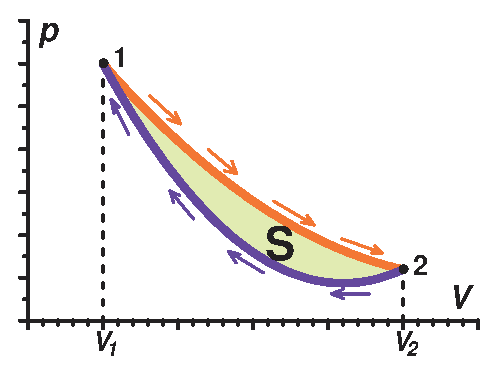
\includegraphics{GP012F09.eps}}
 \put(40,200){\makebox(0,0)[tl]{\parbox{145mm}{
 Если мы пришли из состояния 1 в 2 по какой-то кривой, то работа, совершенная \underline{системой против внешних сил}, положительна:\vspace{-7mm}
 \begin{displaymath}
 \hspace{10mm}A_{1\rightarrow1}=\int\limits_{V_1}^{V_2}p^\prime(V)\;dV\;=S\prime\;>0
 \end{displaymath}
 }}}
 \put(85,160){\makebox(0,0)[tl]{\parbox{100mm}{
 По 1НТД полная энергия системы будет\vspace{-2mm}
 \begin{equation}\label{Eq.A12}
 U_2=U_1+Q_{1\rightarrow2}-A_{1\rightarrow2}\vspace*{-3mm}
 \end{equation}
 где $Q_{1\rightarrow2}$ -- приток тепла к системе.
 }}}
 \put(40,130){\makebox(0,0)[tl]{\parbox{145mm}{
 Надо теперь вернуться из 2 в 1 (можно по другому пути). Совершенная при этом работа будет отрицательной:\vspace{-2mm}
 \begin{displaymath}
 \hspace{10mm}A_{2\rightarrow1}=
  \int\limits_{V_2}^{V_1}p^{\prime\prime}(V)\;dV\;=-S^{\prime\prime}\;<0
 \end{displaymath}
 }}}
 \put(85,95){\makebox(0,0)[tl]{\parbox{100mm}{
  формально: потому, что идем налево. По смыслу: потому, что совершает работу \underline{не система}, а \underline{внешние силы}.
 }}}
 \put(20,67){\makebox(0,0)[tl]{\parbox{165mm}{
 Снова должно соблюдаться 1НТД $\Rightarrow$ полная энергия системы:\vspace{-4mm}
 \begin{equation}\label{Eq.A21}
  \hspace{15mm}U_1= U_2-Q_{2\rightarrow1}-A_{2\rightarrow1}
 \end{equation}
 }}}
 \put(185,49){\makebox(0,0)[r]{
 где $Q_{2\rightarrow1}$ -- отток тепла от системы на возвратном участке.
 }}
 \put(70,42){\makebox(0,0)[tl]{\parbox{115mm}{
 Сложив уравнения (\ref{Eq.A12}) и (\ref{Eq.A21}), получим:\vspace{-2mm}
 \begin{displaymath}
  \hspace{10mm}A\equiv A_{1\rightarrow2}+A_{2\rightarrow1}=S= Q_{1\rightarrow2}-Q_{2\rightarrow1}
 \end{displaymath}
 }}}
 \put(185,0){\makebox(0,0)[br]{\parbox{100mm}{
т.е., суммарная работа $A$, совершенная системой, численно равна площади $S$, охватываемой графиком цикла и равна
 }}}
 \end{picture}\\
разности подведенного к системе ($Q_{1\rightarrow2}$) и отведенного от нее ($Q_{2\rightarrow1}$) количества тепла.

В этом примере пути $p^\prime(V)$ и $p^{\prime\prime}(V)$ разные, причем первый из них проходит выше $\Rightarrow$ площадь $S$ и, соответственно, работа $A$, положительна. Система превратила некое тепло в работу. Это -- \fbox{\bf прямой цикл}, а изо\-бра\-жен\-ный процесс -- \fbox{\bf тепловая машина}.

Особенности прямого цикла:
\begin{itemize}
\item Чтобы закачать тепло $Q_{1\rightarrow2}$ в систему, должно присутствовать более горячее тело (нагреватель).
\item Чтобы забрать тепло $Q_{2\rightarrow1}$ от системы, должно присутствовать более холодное тело (холодильник).
\item Не все тепло $Q_{1\rightarrow2}$ превращается в работу; некоторая часть его ($Q_{2\rightarrow1}$) должна вернуться вовне. {\bf Коэффициент полезного действия} те\-п\-ло\-вой машины (к.п.д.):\vspace{-5mm}
    \begin{displaymath}
    \eta = \frac{A}{Q_{1\rightarrow2}}=\frac{Q_{1\rightarrow2}-Q_{2\rightarrow1}}{Q_{1\rightarrow2}}
    \end{displaymath}
\end{itemize}
Если возвратный путь $p^{\prime\prime}(V)$ лежит выше прямого  $p^\prime(V)$, то площадь
 $S$ и\\
 \begin{picture}(185,60)(0,0)
 %\put(0,0){\framebox(185,60)[b]{}}
 \put(0,0){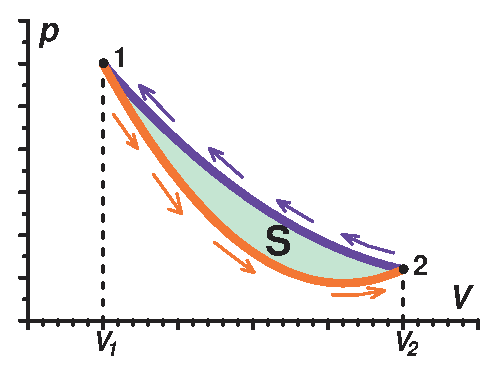
\includegraphics{GP012F10.eps}}
 \put(85,59){\makebox(0,0)[tl]{\parbox{100mm}{
 работа $A$ будут отрицательными. Это значит, что система не тепло превращает в работу, а наоборот -- работу внешних сил превращает в тепло. Раз кривая $p^\prime(V)$ лежит \underline{ниже}, то происходит это расширение при более  \underline{низком} давлении и $\Rightarrow$ при более \underline{низкой} температуре. Но поскольку именно на
 }}}
 \end{picture}\\
 этом этапе система поглощает тепло, то температура нагревателя может быть ниже. Аналогично, сжатие с выделением тепла проходит при более высокой температуре $\Rightarrow$ температура холодильника, забирающего это теп\-ло у системы, может быть выше.

 Такой цикл -- это не прямой, а \fbox{\bf обратный цикл}, а процесс -- не тепловая, а \fbox{\bf холодильная машина}.\\

 Если при термодинамическом процессе теплообмена между системой и окружающим миром нет, то это -- \fbox{\bf адиабатический процесс}. В ре\-аль\-ности либо нужна супер-теплоизоляция, либо процесс должен течь настолько быстро, что теплообмен просто не успел бы произойти.
 \newpage
 В адиабатическом процессе  $\Delta U + \Delta A =0$ (поскольку $\Delta Q\equiv0$).\\
 Если система совершает работу, то \hspace{15mm}$\Delta A > 0\;\;\;\Rightarrow\;\;\;\Delta U<0$.\\
 Если над системой совершают работу, то $\Delta A < 0\;\;\;\Rightarrow\;\;\;\Delta U>0$.\\
 Рассмотрим расширение 1 моля идеального газа:
 \begin{displaymath}
 \Delta A = p\;\Delta V;\hspace{10mm}
 U=\frac{i}2 kT\; N = \frac{i}2RT = C_V\;T
 \hspace{10mm}\Rightarrow\;\;\Delta U=C_V\;\Delta T
 \end{displaymath}
 тогда при \underline{адиабатическом} расширении:
 $C_V\;\Delta T + p\;\Delta V = 0.$\\
 Отсюда следует:
 \begin{itemize}
 \item при адиабатич. расширении $\Delta V>0\;\;\;\Rightarrow\;\;\;\Delta T<0$ (газ охлаждается)
 \item при адиабатическом сжатии $\Delta V<0\;\;\;\Rightarrow\;\;\;\Delta T>0$ (газ нагревается)
 \end{itemize}
 Поскольку для идеального газа $pV=RT$, то получаем диф. уравнение:
 \begin{displaymath}
  \frac{dV}{V}=-\frac{C_V}{R}\cdot\frac{dT}{T}\hspace{10mm}\texttt{или}\hspace{10mm}
  d\left(\frac{R}{C_V}\;\ln V\right)=-d\left(\ln T\right)
 \end{displaymath}
 Его решение -- это\vspace{-5mm}
 \begin{displaymath}
 T\cdot V^{\frac{R}{C_V}}={\rm const.}
 \end{displaymath}

  Вспомним, что $C_p=C_V+R$ и обозначим $C_p/C_V\equiv\gamma$. \\
  Тогда $R/C_V=\gamma-1$, и можно решение переписать как
 \begin{displaymath}
 T\cdot V^{\gamma-1}={\rm const.}\hspace{10mm}\texttt{или}\hspace{10mm}
  p\cdot V^{\gamma}={\rm const.}\hspace{10mm}(\texttt{поскольку}\hspace{5mm}
  p\;V=R\;T).
 \end{displaymath}
Эта формула Пуассона заменяет для адиабатического процесса закон Бойля-Мариотта.

 При адиабатическом переходе из состояния 1 в сост. 2
 \begin{displaymath}
 \frac{T_2}{T_1}=\left(\frac{V_1}{V_2}\right)^{\gamma-1}\hspace{10mm}
 \texttt{или}\hspace{10mm} \frac{p_2}{p_1}=\left(\frac{V_1}{V_2}\right)^{\gamma}
 \end{displaymath}
 тогда как при изотермическом переходе\vspace{-4mm}
 \begin{displaymath}
 p\;V={\rm const.}\hspace{10mm}\texttt{и}\hspace{10mm} \frac{p_2}{p_1}=\frac{V_1}{V_2}
 \end{displaymath}

Можно считать, что и {\bf адиабата}, и {\bf изотерма} -- это как бы частные случаи \fbox{\bf политропы}, причем для изотермы показатель политропы $\gamma=1$, а для адиабаты $\gamma=C_p/C_V>1$.\\
 \begin{picture}(185,65)(0,0)
 %\put(0,0){\framebox(185,65)[b]{}}
 \put(0,0){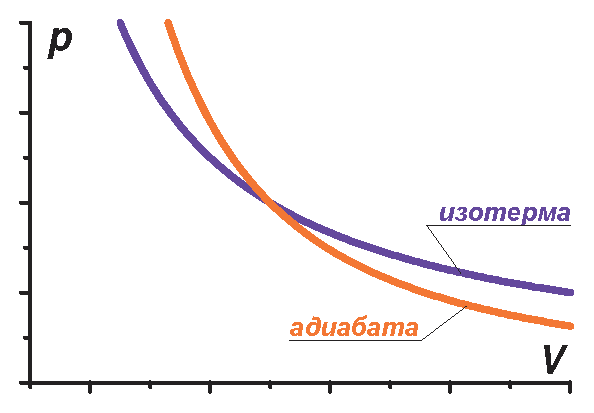
\includegraphics{GP012F11.eps}}
 \put(100,66){\makebox(0,0)[tl]{\parbox{85mm}{
Вообще-то, в природе не бывает истинных адиабат и изотерм, поскольку невозможно идеально теплоизолировать систему, как и обеспечить 100\% тепловой контакт. На самом деле, есть только политропы. Если $\gamma\simeq1$, то это близко к изотерме, а если $\gamma\simeq C_p/C_V$, то к адиабате.
 }}}
 \end{picture}\\
Кривая адиабатического процесса идет круче, чем изотермического.\\
Объяснение простое: при расширении давление уменьшается, но при этом происходит остывание газа, и из-за этого давление падает еще больше.

Пример: азот при н.у. сжимают в 5 раз адиабатически или изотермически. Разница -- ?
Решение: азот = N$_2 \Rightarrow$ i=5 степеней свободы $\Rightarrow \gamma =(i+2)/i =7/5=1.4$. \begin{itemize}
\item изотермически:
       \begin{displaymath}
       \frac{p_5}{p_1}=\frac{V_1}{V_5}\hspace{10mm}\Rightarrow\hspace{10mm}
       p_5=p_1\;\frac{V_1}{V_5}=1{\rm am}\cdot 5 = 5{\rm am}
       \end{displaymath}
\item адиабатически:
       \begin{displaymath}
       \frac{p_5}{p_1}=\left(\frac{V_1}{V_5}\right)^{1.4}\hspace{10mm}\Rightarrow\hspace{10mm}
       p_5=1{\rm am}\cdot 5^{1.4} = 9.52{\rm am}
       \end{displaymath}
       \begin{displaymath}
       \frac{T_5}{T_1}=\frac{V_1}{V_5}\hspace{10mm}\Rightarrow\hspace{10mm}
       T_5=T_1\cdot\left(\frac{V_1}{V_5}\right)^{\gamma-1}=
       300{\rm K}\cdot 5^{0.4} = 571{\rm K}=298^\circ{\rm C}
       \end{displaymath}
\item а если адиабатически сжать не в 5, а в 20 раз?
       \begin{displaymath}
       \frac{p_{20}}{p_1}=\left(\frac{V_1}{V_{20}}\right)^{1.4}\hspace{10mm}\Rightarrow\hspace{10mm}
       p_{20}=1{\rm am}\cdot 20^{1.4} = 66.3{\rm am}
       \end{displaymath}
       \begin{displaymath}
       \frac{T_{20}}{T_1}=\frac{V_1}{V_{20}}\hspace{10mm}\Rightarrow\hspace{10mm}
       T_{20}=T_1\cdot\left(\frac{V_1}{V_{20}}\right)^{\gamma-1}=
       300{\rm K}\cdot 20^{0.4} = 994{\rm K}=721^\circ{\rm C}
       \end{displaymath}
       Двигатель Дизеля! (Rudolf Diesel, 1897, Berlin)
\end{itemize}
 \begin{picture}(185,60)(0,0)
 %\put(0,0){\framebox(185,60)[b]{}}
 \put(0,0){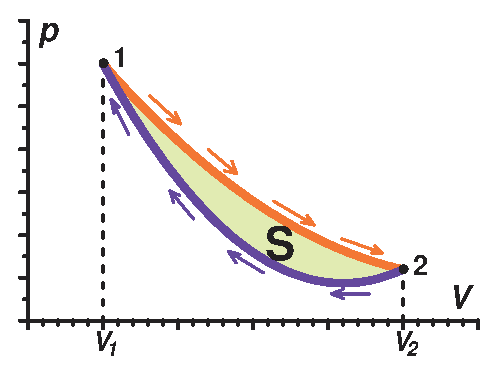
\includegraphics{GP012F09.eps}}
 \put(80,59){\makebox(0,0)[tl]{\parbox{105mm}{
  Как мы видели, для тепловой машины с прямым циклом только часть тепла, пе\-ре\-да\-ва\-е\-мо\-го ей нагревателем, пре\-вра\-ща\-ет\-ся в работу; остальная же часть возвращается холодильнику. КПД при этом равен\vspace{-5mm}
    \begin{displaymath}
    \hspace{10mm}\eta = \frac{A}{Q_{1\rightarrow2}}=\frac{Q_{1\rightarrow2}-Q_{2\rightarrow1}}{Q_{1\rightarrow2}}
    \end{displaymath}
 }}}
 \end{picture}\\
Хотелось бы, чтоб $\eta\rightarrow1$, и тогда бы $Q_{2\rightarrow1}=0$, ничего не пришлось бы возвращать холодильнику, и он вообще стал бы не нужен! Получился бы двигатель, который просто все тепло окружающей среды превращал бы в работу ({\sl perpetuum mobile II рода}).

Но долгое время ничего не получалось. В 1824 г. Сади Карно: {\sl ``Раз\-мыш\-ления о движущей силе огня и о машинах, способных развивать эту силу''}. (Nicolas Leonard Sadi Carnot, 1796-1832, Paris). Умер от холеры, все было сожжено, больше никаких его работ не сохранилось. Главный вывод: избежать возврата $Q_{2\rightarrow1}$ невозможно.

Позднее Клаузиус и Томсон это обобщили и получили 2НТД:\\ {\bf невозможен такой периодический цикл, единственным ре\-зуль\-та\-том которого было бы получение работы за счет взятого количества тепла от одного источника.}

Другая формулировка: {\bf невозможен perpetuum mobile II рода.}\\

Тем не менее, надо к этому стремиться!  В своих ``Размышлениях'' Карно рассмотрел цикл, который теперь так и называется: \fbox{\bf цикл Карно}.
Займемся им подробнее. Цикл Карно -- это 2 изотермы и 2 адиабаты.
Идеальных изотерм и адиабат не бывает, но мы пока про это забудем. Почему вообще ИЗОТЕРМЫ? Потому что просто в это время $T_\texttt{газа}=T_\texttt{нагревателя}=$ const. Почему вообще АДИАБАТЫ? Потому что это -- противоположность изотерм (в смысле теплообмена). И вообще, если никаких специальных хитростей не выдумывать, то в природе могут быть только политропы --- все, что между изотермами и адиабатами.

 Для осуществления цикла Карно нам нужен нагреватель с темпера\-ту\-рой $T_1$, подводящий к газу тепло и заставляющий его расширяться изотермически, а также холодильник с температурой $T_3$, забирающий выделяющееся тепло при изотермическом сжатии.\\
 \begin{picture}(185,110)(0,0)
 %\put(0,0){\framebox(185,110)[b]{}}
 \put(10,0){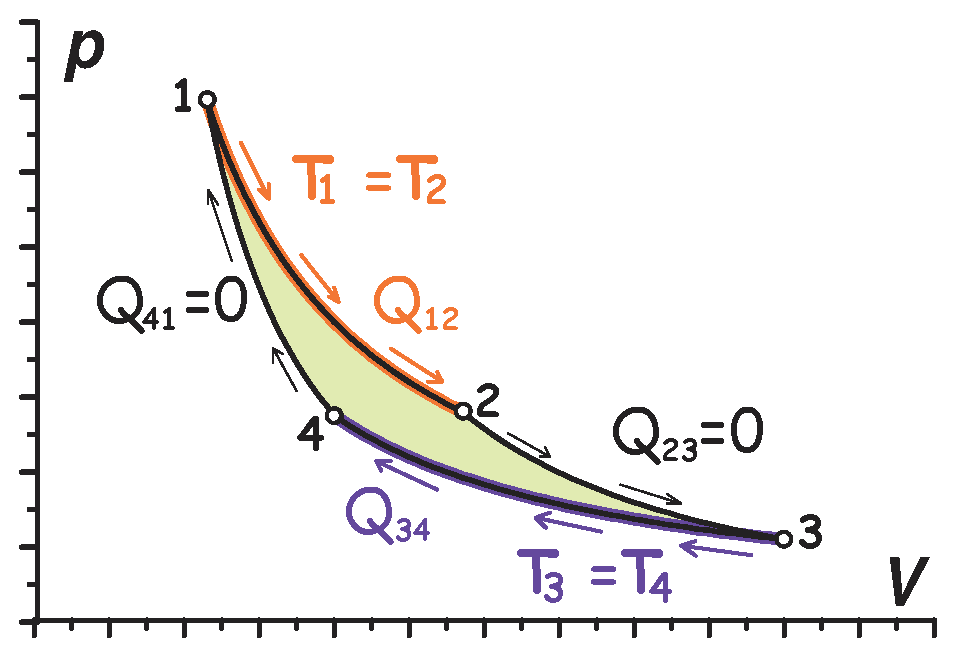
\includegraphics{GP012F12.eps}}
 \put(100,105){\makebox(0,0)[tl]{\parbox{85mm}{
 (На адиабатических участках нет передачи тепла, поэтому там ни нагреватель, ни холодильник не нужны). }}}
 \end{picture}\\
Итак, пусть 1 моль идеального газа  -- в состоянии 1 при $p_1,V_1,T_1$.
\begin{enumerate}
\item Будем с помощью нагревателя поддерживать его при $T_1$ и дадим ему расширяться (изотермически) до состояния 2. На участке 1-2 газ получит тепло $Q_{12}$ и совершит работу $A_{12}=Q_{12}$. (Поскольку $T_1=T_2$, и газ -- идеальный, то $U=$ const.)
\item В точке 2 перестанем подогревать газ и разрешим ему расширяться адиабатически (без теплообмена) до точки 3. При этом он остынет до $T_3$ и совершит еще какую-то работу $A_{23}$.
\item Теперь начнем изотермически сжимать газ, а появляющееся тепло отводить с помощью холодильника. На пути 3-4 газ отдаст тепло $Q_{34}$ и над ним совершится работа $A_{34}=Q_{34}$. (Снова $U=$ const.)
\item В точке 4 продолжим сжимать газ, но уже без отвода тепла. Для этого потребуется еще какая-то работа $A_{41}$, и газ нагреется до $T_1$.
\end{enumerate}
В итоге, газ получит тепло\vspace{-12mm}
\begin{displaymath}
\hspace{20mm}Q_\Sigma=Q_{12}-Q_{34}\;,
\end{displaymath}
а совершенная им суммарная работа, по 1НТД равная $Q_\Sigma$,  составит
\begin{displaymath}
A_\Sigma=Q_\Sigma=A_{12}+A_{23}-A_{34}-A_{41}\;.
\end{displaymath}
Вспомнив, что  $A_{12}=Q_{12}$, а $A_{34}=Q_{34}$, с удивлением обнаружим, что
\begin{displaymath}
A_{23}=A_{41}\;,
\end{displaymath}
то есть, что в цикле Карно работа газа и работа внешних сил на адиа\-ба\-ти\-чес\-ких участках 2-3 и 4-1 компенсируют друг друга. (Это и в самом деле так; можно доказать через соответствующие интегралы).

Если же посчитать работу на изотермических участках 1-2 и 3-4, то получим:\vspace{-5mm}
\begin{displaymath}
\hspace{10mm}A_{12}=\int\limits_{V_1}^{V_2}p(V)\;dV=
\int\limits_{V_1}^{V_2}\frac{R\;T_1}{V}\;dV=
R\;T_1\left(\ln V_2-\ln V_1\right)=
R\;T_1\;\ln \frac{V_2}{V_1}\;.
\end{displaymath}
Аналогично,\vspace{-5mm}
\begin{displaymath}
-A_{34}=\int\limits_{V_3}^{V_4}p(V)\;dV=
R\;T_3\;\ln \frac{V_4}{V_3}\;.
\end{displaymath}
Но мы знаем, что при адиабатических переходах\vspace{-14mm}
\begin{displaymath}
\hspace{140mm}\frac{T_a}{T_b}=\left(\frac{V_b}{V_a}\right)^{\gamma-1}
\end{displaymath}
поэтому
\begin{displaymath}
\hspace{10mm}\left(\frac{V_4}{V_1}\right)^{\gamma-1}=
\frac{T_1=T_2}{T_4=T_3}=\left(\frac{V_3}{V_2}\right)^{\gamma-1}
\hspace{10mm}\Rightarrow\hspace{10mm}\frac{V_4}{V_1}=\frac{V_3}{V_2}
\hspace{10mm}\Rightarrow\hspace{10mm}\frac{V_4}{V_3}=\frac{V_1}{V_2}
\end{displaymath}
КПД цикла Карно равен\vspace{-5mm}
\begin{displaymath}
\hspace{40mm}\eta=\frac{A_\Sigma}{Q_{12}}=\frac{A_{12}-A_{34}}{A_{12}}=\frac{T_1-T_3}{T_1}
\end{displaymath}
и зависит только от разности температур нагревателя и холодильника!\\

Замечание: цикл Карно -- идеализированный. Он -- для идеального газа; он -- для равновесных процессов $\Rightarrow$ для обратимых процессов. В жизни все сложнее, и КПД только хуже. Поэтому цикл Карно надо рас\-смат\-ри\-вать как ВЕРХНИЙ ПРЕДЕЛ для тепловых машин.\\

Любой произвольный цикл = набору $k$ циклов Карно. $\forall\; k$-го цикла $T_{1k}\leq T_{\rm max}$ и $T_{2k}\geq T_{\rm min}$, поэтому как $\forall\; k$, так и для ВСЕГО цикла вцелом
\begin{displaymath}
\eta\leq\frac{T_{\rm max}-T_{\rm min}}{T_{\rm max}}
\end{displaymath}
 \begin{picture}(190,210)(0,0)
 %\put(0,0){\framebox(190,210)[b]{}}
 \put(0,105){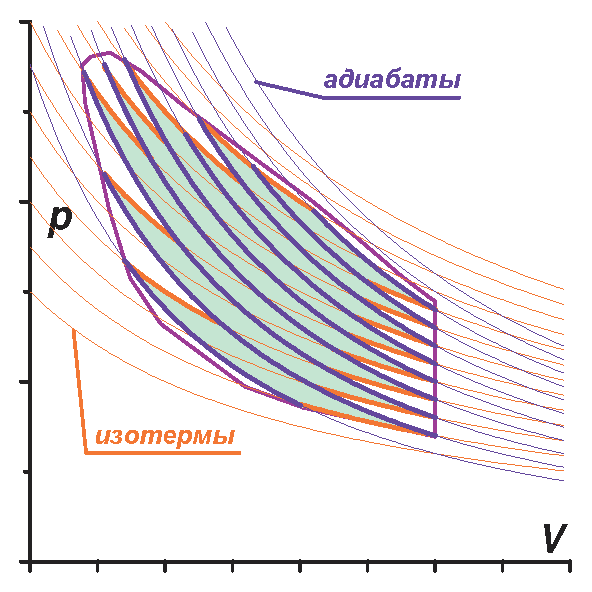
\includegraphics{GP012F13.eps}}
 \put(98,105){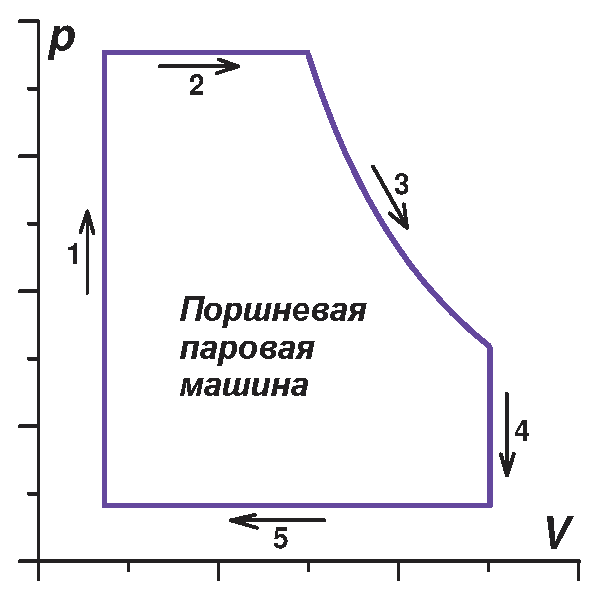
\includegraphics{GP012F14.eps}}
 \put(0,0){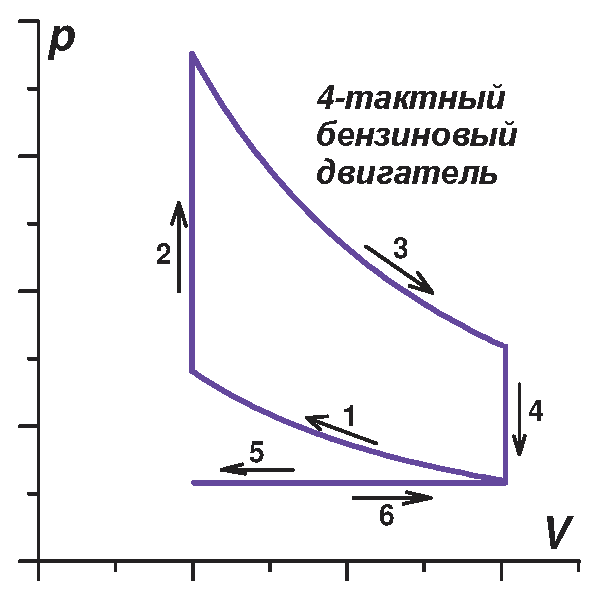
\includegraphics{GP012F15.eps}}
 \put(98,0){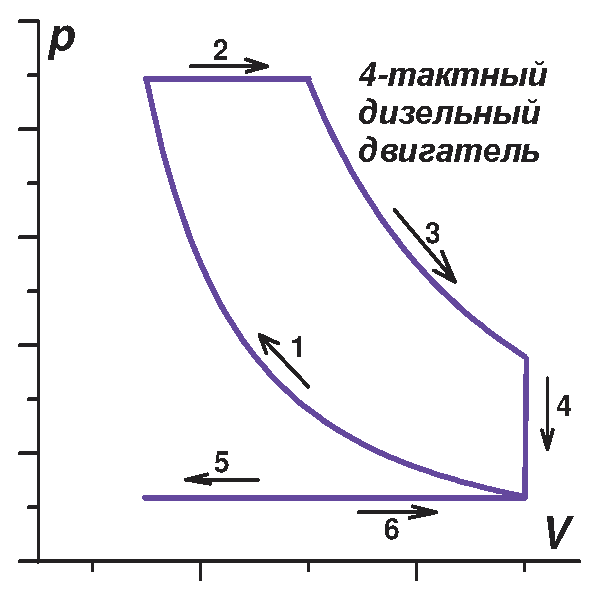
\includegraphics{GP012F16.eps}}
 \end{picture}\\
 \begin{picture}(190,90)(0,0)
 %\put(0,0){\framebox(190,90)[b]{}}
 \put(10,0){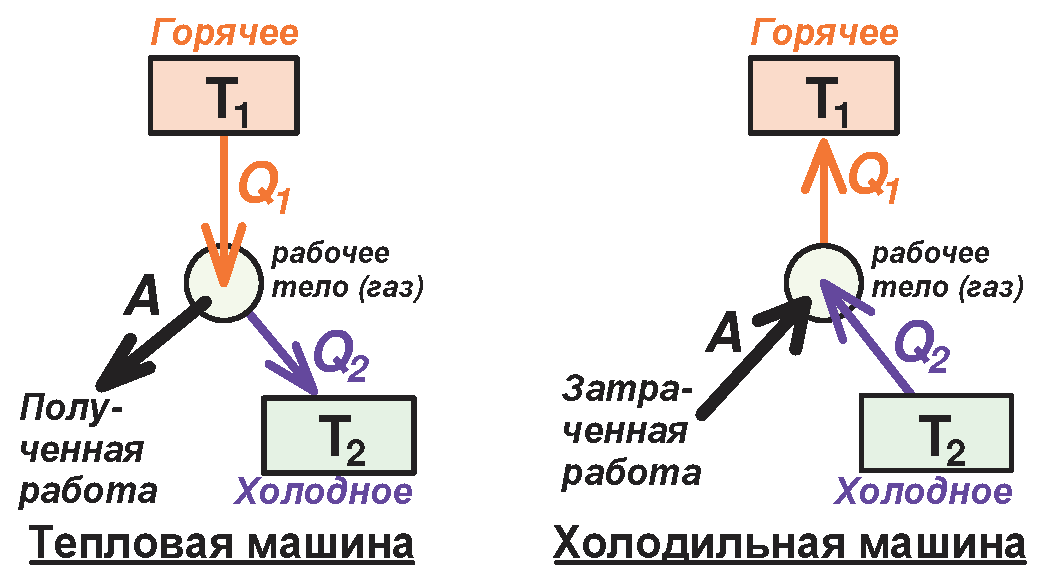
\includegraphics{GP012F20.eps}}
 \end{picture}\\

Для обратимого цикла Карно:
\begin{displaymath}
\eta=\frac{T_1-T_2}{T_1};\hspace{10mm}A=\eta\cdot Q_1;
\hspace{10mm}Q_2=Q_1-A=(1-\eta)\cdot Q_1=\frac{T_2}{T_1}\cdot Q_1
\end{displaymath}
откуда получаем интересное соотношение:
\begin{displaymath}
\frac{Q_2}{T_2}=\frac{Q_1}{T_1}
\end{displaymath}
Если передаваемую в каком-то процессе от тела к телу величину $S=Q/T$ назвать, например, ``приведенным количеством тепла'', то можно сказать, что в случае идеального обратимого цикла Карно приведенное количество тепла, получаемое рабочим телом (не важно -- от нагревателя или от холодильника), равно приведенному количеству тепла, отдаваемому ра\-бо\-чим телом (опять-таки, не важно, куда). Какой в этом смысл?... Если при\-ход ЧЕГО-ТО = расходу ЧЕГО-ТО, то ЭТО сохраняется.\\
Это таинственная величина -- ЭНТРОПИЯ.

Можно показать, что для НЕидеального цикла получаемое ЭТО > отдаваемого. Вообще, не только для циклов, но и для любых процессов в замкнутой системе энтропия НЕ УБЫВАЕТ (для обратимых процессов -- остается постоянной).
\newpage
\underline{\bf Свойства ЭНТРОПИИ.}
\begin{itemize}
 \item Для любого (не кругового) процесса $A\rightarrow B$ энтропия системы изменяется на величину
     \begin{displaymath}
     \int\limits_A^B\frac{dQ}{T}\hspace{10mm}\Rightarrow\hspace{10mm}
     S_B=S_A+\int\limits_A^B\frac{dQ}{T}
     \end{displaymath}
     где под $Q$ понимается тепло, ПОЛУЧЕННОЕ системой.
 \item Для кругового обратимого процесса (обратимого цикла) $A\rightarrow B\rightarrow A$ энтропия системы не меняется:
     \begin{displaymath}
     \int\limits_A^B\frac{dQ}{T}+\int\limits_B^A\frac{dQ}{T}=\oint\frac{dQ}{T}=0
     \end{displaymath}
 \item Для кругового НЕобратимого процесса (если там есть хотя бы один НЕобратимый участок) энтропия системы возрастает:
     \begin{displaymath}
     \oint\frac{dQ}{T}>0
     \end{displaymath}
 \item Пример: 100 г воды охлаждаются от 15 то 0$^\circ$C. Как изменится энтропия?\\
     Решение: считая, что объем не изменился, получим $dQ=m\cdot c\cdot dT$, где $m$ -- масса, а $c$ -- удельная теплоемкость. Тогда
     \begin{displaymath}
     S_B-S_A=\int\limits_A^B\frac{dQ}{T}=\int\limits_{T_1}^{T_2}m\;c\;\frac{dT}{T}=
     m\;c\;\ln\left(\frac{T_2}{T_1}\right)=
     \end{displaymath}
     \begin{displaymath}
     =100\texttt{ г }\cdot1\texttt{ кал/г/град }\cdot\ln\frac{273}{288}=-5.34\texttt{ кал/град}
     \end{displaymath}
     минус получился потому, что энтропия уменьшилась!
  \item Для ЗАМКНУТОЙ системы она уменьшиться не может.
  \item Это все были слова об ИЗМЕНЕНИИ энтропии. А сама она чему равна? Теорема Нернста (3НТД):
      \begin{center}
      \fbox{$S(T\rightarrow0)=0$}
      \end{center}
 \end{itemize}

\newpage
\underline{\bf Обратимые процессы:}\\
 \begin{picture}(190,70)(0,0)
 %\put(0,0){\framebox(190,70)[b]{}}
 \put(0,0){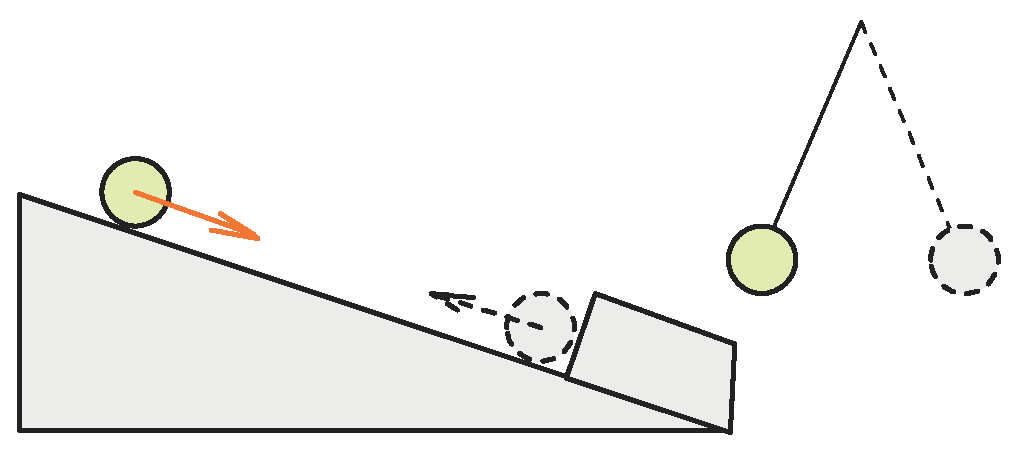
\includegraphics{GP012F17.eps}}
 \end{picture}\\
Упругий шарик; маятник без трения; Цикл Карно; движение одной молекулы; ...\\
\underline{\bf Необратимые процессы:}\\

{\bf Необратимым является такой процесс, обратный которому может протекать лишь как звено более сложного процесса.}\\

Для необратимого процесса характерно его {\bf направление}. \\
В {\bf положительном} направлении процесс течет ``сам собой'' \\
Работа $\longrightarrow$ тепло (когда есть трение или неупругие процессы, т.е. ВСЕГДА).\\
Перенос тепла от горячего тела к холодному.\\
Расширение газа в пустоту (убираем перегородку):\\
 \begin{picture}(190,32)(0,0)
 %\put(0,0){\framebox(190,32)[b]{}}
 \put(10,0){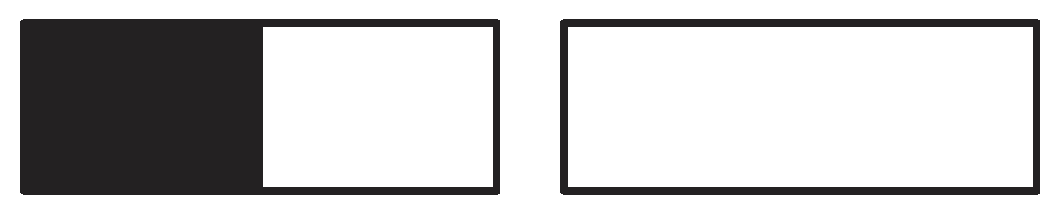
\includegraphics{GP012F18.eps}}
 \end{picture}\\
Чтобы загнать газ назад, нужно совершить работу по его сжатию. \\
И вообще: переход в {\bf отрицательном} направлении требует дополнительных внешних усилий, то есть, должен быть еще какой-то внешний процесс. Так, чтобы перегнать тепло от холодного к горячему (холодильная машина), нужен дополнительный положительный процесс, который совершил бы работу (она потом в виде тепла передается негревателю).

Вопрос: почему движение одной молекулы -- обратимо, а многих молекул -- нет?

Ответ: по законам статистики.\\
 \begin{picture}(190,35)(0,0)
 %\put(0,0){\framebox(190,32)[b]{}}
 \put(10,0){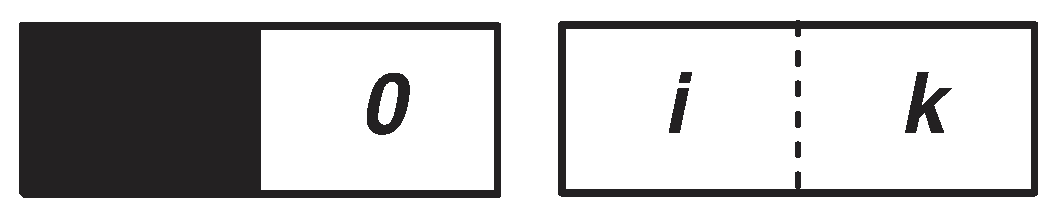
\includegraphics{GP012F19.eps}}
 \end{picture}\\
Пусть слева было $n$ молекул, а справа 0. После убирания перегородки все перемешалось. Какова вероятность, что слева будет $i$, а справа $j$? Если фазовые объемы и плотность вероятности слева и справа равны, то для КАЖДОЙ молекулы вероятность быть слева или справа = по 50\%. Ну, например, $n=4$. Присвоим молекулам имена: A, B, C, D -- и посмотрим, какие могут быть варианты:\\
\parbox{95mm}{
\begin{tabular}{|cccc|cccc|c|c|c|}\hline
\multicolumn{4}{|c|}{слева}&\multicolumn{4}{|c|}{справа}&i&j&$W_i$\\ \hline
A&B&C&D& & & & &4&0&1\\ \hline
A&B&C& & & & &D&3&1& \\
A&B& &D& & &C& &3&1& \\
A& &C&D& &B& & &3&1& \\
 &B&C&D&A& & & &3&1&4\\ \hline
A&B& & & & &C&D&2&2& \\
A& &C& & &B& &D&2&2& \\
 &B&C& &A& & &D&2&2& \\
A& & &D& &B&C& &2&2& \\
 &B& &D&A& &C& &2&2& \\
 & &C&D&A&B& & &2&2&6\\ \hline
A& & & & &B&C&D&1&3& \\
 &B& & &A& &C&D&1&3& \\
 & &C& &A&B& &D&1&3& \\
 & & &D& &B& & &1&3&4\\ \hline
 & & & &A&B&C&D&0&4&1\\ \hline
\end{tabular}
}\parbox{95mm}{Всего получилось 16 возможностей ($16=2^n$). Наиболее вероятен случай, когда $i=j=n/2$: 6/16=37.5\%. $W_i$ -- термодинамическая вероятность (число микросостояний). Случай, когда все 4 молекулы сами собой соберутся в левой половине, -- только ОДИН: 1/16$\simeq$6\%.
Если бы у нас было не 4 молекулы а, например, $n=10$, этот шанс еще уменьшился бы:
\begin{displaymath}
w=\frac{1}{2^{10}}=\frac{1}{1024}\simeq0.1\%
\end{displaymath}
А про МАКРО-количество и говорить нечего: при $n=10^{19}$
\begin{displaymath}
w=\frac{1}{2^{10\,000\,000\,000\,000\,000\,000}}
\end{displaymath}
}\\

Необратимый процесс -- такой, обратный которому \underline{\bf маловероятен}.
Вообще-то, кроме координат молекул надо и их скорости учитывать (вместо распределения по объему рассматривать распределение по ФАЗОВОМУ объему). Из статистики известно: система, предоставленная самой себе, стремится прийти к макросостоянию $i$, которое реализуется максимальным числом способов, т.е., к состоянию с максимальной $W_i$. Если вместо $W_i$ использовать $S\equiv k\cdot\ln W_i$, то это уже будет аддитивная величина: при разбивке системы A на 2 системы B и C, $W_A=W_B\cdot W_C$, но $S_A=S_B+S_C$! И оказывается, что определенная таким способом вел-на $S$ есть ни что иное, как ЭНТРОПИЯ! (Больцман доказал)\\

\noindent
\begin{tabular}{rcl}
Упорядоченное движение &\rule{0mm}{11mm}
 $\stackrel{\texttt{флуктуации}}{\rule[1.3mm]{30mm}{0.2mm}\!\!\rightarrow}$
 & неупорядоченное движение\\
\color{blue}
Движение тела как целого &\rule{0mm}{11mm}
 $\stackrel{\texttt{\color{blue}трение}}{\rule[1.2mm]{20mm}{0.2mm}\!\!\rightarrow}$
 & \color{blue}нагрев\\
Упорядоченное положение &\rule{0mm}{15mm}
 $\stackrel{\texttt{флуктуации}}{\rule[1.3mm]{30mm}{0.2mm}\!\!\rightarrow}$
 & неупорядоченное положение\\
\color{red}
Неоднородная смесь &\rule{0mm}{11mm}
 $\stackrel{\texttt{\color{red}диффузия}}{\rule[1.2mm]{20mm}{0.2mm}\!\!\rightarrow}$
 & \color{red}однородная смесь\\
\end{tabular}\\[5mm]

\centerline{\fbox{2НТД носит статистический характер.}}

Броуновские частицы настолько малы, что уже не подчиняются 2НТД. И вообще, ТЕРМОДИНАМИКА -- для \underline{\bf больших} статистических ансамблей.

В космических масштабах она тоже неприменима: кто сказал, что Вселенная -- это замкнутая система, что в ней должно быть равновесие, и что вообще наши модели можно рас\-про\-стра\-нять на нее? (``Тепловая смерть'' Вселенной)
\end{document}
